%%%%%%%%%%%%%%%%%%%%%%%%%BORRAR
\documentclass[a4paper]{article}
\usepackage[utf8]{inputenc}
\usepackage[spanish, es-tabla]{babel}

\usepackage[a4paper, footnotesep = 1cm, width=18cm, left=2cm, top=2.5cm, height=25cm, textwidth=18cm, textheight=25cm]{geometry}
%\geometry{showframe}

\usepackage{tikz}
\usepackage{amsmath}
\usepackage{amsfonts}
\usepackage{amssymb}
\usepackage{float}
\usepackage{graphicx}
\usepackage{caption}
\usepackage{subcaption}
\usepackage{multicol}
\usepackage{multirow}
\setlength{\doublerulesep}{\arrayrulewidth}
\usepackage{xcolor}

\usepackage{hyperref}
\hypersetup{
    colorlinks=true,
    linkcolor=blue,
    filecolor=magenta,      
    urlcolor=blue,
    citecolor=blue,    
}

\newcommand{\quotes}[1]{``#1''}
\usepackage{array}
\newcolumntype{C}[1]{>{\centering\let\newline\\\arraybackslash\hspace{0pt}}m{#1}}
\usepackage[american]{circuitikz}
\usepackage{fancyhdr}
\usepackage{units} 

\pagestyle{fancy}
\fancyhf{}
\lhead{22.13 Electrónica III}
\rhead{Mechoulam, Lambertucci, Martorell, Londero}
\rfoot{\center \thepage}
\begin{document}
\section{auxiliar}
\tableofcontents
%%%%%%%%%%%%%%%%%%%%%%%%%BORRAR

\subsection{Introducción}

Los mandos de control o actualmente llamados \quotes{Joysticks} son parte fundamental de varios dispositivos electrónicos utilizados hoy en día. Consolas de videojuegos, sillas de ruedas eléctricas, aeronaves radio-controladas e incluso hasta cohetes de la NASA. En su forma más básica, un potenciómetro, los mandos de control revolucionaron al rededor de finales de la segunda guerra mundial la manera de controlar dispositivos digitales de manera analógica. 

En esta sección del informe nos centraremos en la implementación de un convertidor analógico a digital mediante el uso del Joystick HW-504 junto a la investigación realizada.

\subsection{Joystick HW-504}

El mando de control a utilizar está compuesto por dos potenciómetros, uno para el eje X y otro para el eje Y, y un switch accionado al apretar el mando hacia dentro. El periférico requiere de una alimentación de $5V$ y puede esquematizarse como el siguiente modelo electóonico:

\begin{figure}[H]
	\begin{subfigure}[t]{0.49\textwidth}
		\centering
		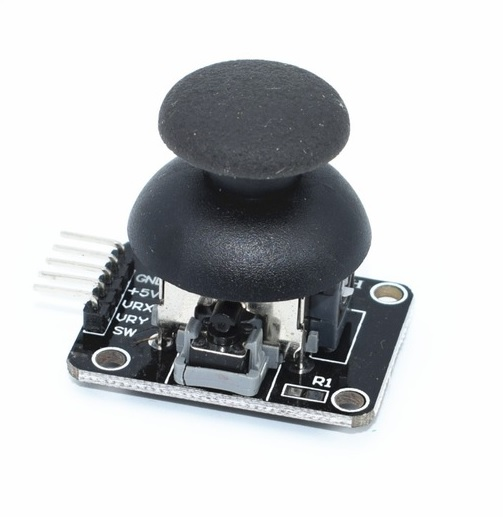
\includegraphics[width=0.6\textwidth]{ImagenesEjercicio8/joystick.jpg}
		\caption{Mando de control HW-504 a utilizar$^{0}$.}
		\label{fig:joystick}
	\end{subfigure}
	\begin{subfigure}[t]{0.49\textwidth}
		\centering
		\scalebox{0.7}{
		\begin{circuitikz}

		\draw

		(-3,0) node[label=west:{\color{blue}\textbf{+5V}}](5V){}
			to[short,o-*] ++ (2, 0)
			node[](LEFT_POTX_NODE){}
	
		(LEFT_POTX_NODE) to[pR, -*, name=pot-x] ++ (5, 0)
			node[](RIGHT_POTX_NODE){}

		(pot-x.wiper) to[short, -o] ++ (0, 0)
			node[label=north:{\color{blue}\textbf{VRx}}](){}

		(LEFT_POTX_NODE) to[short, -*] ++ (0, -2)
			node[](LEFT_POTY_NODE){}
			to[pR, -*, name=pot-y] ++ (5, 0)
	
		(pot-y.wiper) to[short, -o] ++ (0,0)
			node[label=north:{\color{blue}\textbf{VRy}}](){}
	
		(LEFT_POTY_NODE) to[short] ++ (0, -1.7)
			node[](LEFT_SW_NODE){}
			to[push button] ++ (5, 0)
			to[short, -o] ++ (2,0)
			node[label=east:{\color{blue}\textbf{SW}}](SW){}
	
		(RIGHT_POTX_NODE) to[short] ++ (0, -2)

		(RIGHT_POTX_NODE) to[short, -o] ++ (2, 0)
	
			node[label=east:{\color{blue}\textbf{GND}}]{}
			
		to[open] ++ (0, -5.5)

		;

		\end{circuitikz}
		}
		\caption{Circuito equivalente del mando HW-504 con mismos nombres que el pin-out del periférico.}
		\label{circuit:joytick_eq}
	\end{subfigure}
\end{figure}

\footnotetext{https://eshop.tecnoconciencia.com.ve/eshop/wp-content/uploads/2017/08/JOYSTICK-ARDUINO.jpg. [Accessed: 23- Sep- 2019].}

\subsection{circuitikz que en algun momento vamos ausar saludos}

\begin{figure}[H]

	\centering
	\begin{circuitikz}
		\draw	
	
			node[op amp](opamp){}
			
			(opamp.up) to[short, -*] ++ (0, 2)
				to[open] ++ (-4, 0)
				node[label=west:$V_{CC}$]{}
				to[short, o-] ++ (8, 0)
			
			(opamp.down) to[short, -*] ++ (0, -2)
				to[open] ++ (-4, 0)
				node[label=west:$GND$]{}
				to[short, o-] ++ (8, 0)
				
			(opamp.-) to[short] ++ (-0.5, 0)
				node[label=west:$V_{REF}$]{}				
				to[R, l=$R_1$, *-*] ++ (0, 2)
				to[open] ++ (0, -2)
				to[short] ++ (0, -1)
				to[R, l=$R_2$, -*] ++ (0, -2.03)			
			
			(opamp.+) to[short] ++ (-1, 0)
				to[short, -o] ++ (-2, 0)
				node[label=west:$V_{in}$]{}
	
			(opamp.out) to[short, -o] ++ (2.75, 0)
				node[label=east:$V_{out}$]{}
	
		;
	\end{circuitikz}
	\caption{Amplificador operacional en configuración comparador.}
	\label{circ:comparador}
\end{figure}


\begin{equation*}
V_{out} = A_0 (V_{in} - V_{REF}) =
\left\{
\begin{aligned}
		& \approx V_{CC} \ \ \ \ \ si \ \ V_{in} > V_{REF} \\		
		& \approx 0 \ \ \ \ \ \ \ \ \ si \ \ V_{in} < V_{REF}\\		
\end{aligned}
\right.
\end{equation*}

\begin{figure}[H]
	\centering
	\begin{circuitikz}
		\draw	
		
		%%%%%%%%%%%%%%%%%%%%%%%%%%%%%%%%%%%%%%%%%%%%%%%%%%%%%%%%%%%%
		%Setting figures
		%%%%%%%%%%%%%%%%%%%%%%%%%%%%%%%%%%%%%%%%%%%%%%%%%%%%%%%%%%%%
		node[op amp](op1){} %Opamp1
			to[open] ++ (-0.1, -0.3)
			node[label=\tiny{Comparator}]{}
			to[open] ++ (0,0.2)
		to[open] ++ (0, -3)
		
		node[op amp, yscale=-1](op2){} %Opamp2
			to[open] ++ (-0.1, -0.3)
			node[label=\tiny{Comparator}]{}
			to[open] ++ (0,0.2)
		to[open] ++ (3, 1.5)
		
		node[fourport](srlatch){} %SR-Latch
			(srlatch.1) ++ (0.3, -0.3) node[label=$S$]{}
			(srlatch.2) ++ (-0.3, -0.3) node[label=$\overline{Q}$]{}
			(srlatch.3) ++ (-0.3, -0.3) node[label=$Q$]{}
			(srlatch.4) ++ (0.3, -0.3) node[label=$R$]{}
		to[open] ++ (4, 2)
		
		node[npn](npn){} %Neperiano
			(npn.E) node[tlground]{}

		(srlatch.2) ++ (2.5, 0) node[fourport, label=center:OUT, scale = 0.5](outdriver){}
		%%%%%%%%%%%%%%%%%%%%%%%%%%%%%%%%%%%%%%%%%%%%%%%%%%%%%%%%%%%%
		%NODES:
		%	op1, op2, srlatch, npn, outdriver
		%
		%%%%%%%%%%%%%%%%%%%%%%%%%%%%%%%%%%%%%%%%%%%%%%%%%%%%%%%%%%%%
		(op1.out) |- (srlatch.4)
		
		(op2.out) |- (srlatch.1)
		
		(srlatch.3) to[short] ++ (0.5, 0)
			node[plain crossing, rotate=45]{}
		
		(srlatch.2) to[short, o-o] (outdriver.west)
			to[open, -*] ++ (-1, 0)
			|- (npn.B)
			
		(npn.C) to[short, -o] ++ (0, 1.75)
			node[label=north:DISCHARGE]{}
			node[label=west:7]{}
			
		(outdriver.east) to[short, -o] ++ (2, 0)
			node[label=east:OUT]{}
			node[label=north:3]{}
			
		(srlatch.north) to[short, o-o] ++ (0, 3.75)
			node[label=north:RESET]{}
			node[label=west:4]{}
		
		(op1.-) to[short, -*] ++ (-0.5, 0)
			to[short] ++ (0, 2.5)
			node[ocirc, label=north:CONTROL VOLT]{}
			node[label=west:5]{}		
			to[open] ++ (0, -2.5)
			to[short, -*] ++ (-2.5, 0)
			to[R, l_=$5K$, -o] ++ (0, 2.42)
			node[label=north:VCC]{}
			node[label=west:8]{}
			to[open] ++ (0, -2.42)
			to[R, l=$5K$, -*] ++ (0, -3.1)
			node(aux){}
			to[R, l=$5K$, -o] ++ (0, -3)
			node[label=south:GND]{}
			node[label=west:1]{}


		(op1.+) to[short] ++ (-1.2, 0)
			to[short] ++ (0, 0.5)
			to[short, -o] ++ (-3, 0)
			node[label=north:6]{}
			node[label=west:THRESHOLD]{}

		(op2.+) to[short] ++ (-2.94, 0)
		
		(op2.-) to[short] ++ (-1.2, 0)
			to[short] ++ (0,0.5)
			to[short, -o] ++ (-3, 0)
			node[label=north:2]{}
			node[label=west:TRIGGER]{}
		
		;
	\end{circuitikz}
	\caption{Diagrama en bloques del integrado 555.}
	\label{fig:555}
\end{figure}


\end{document}